%\section{Schedule and Cost Baseline}
\label{sec:schcost}

Cost estimates for engineering, designing, fabricating, assembling, testing, and installing the Heavy Photon Search detector 
are given below. The costs assume considerable savings from the reuse of many parts of the Test Run, which was already assembled 
from silicon microstrip sensors donated by Fermilab, made use of DAQ crates and equipment from SLAC,
and utilized many contributions from JLab, including PbWO$_4$ calorimeter crystals, the chicane and analyzing magnets, magnet power supplies,
and beam diagnostic apparatus. Much of the calorimeter readout electronics utilizes designs which are already in place for the Hall
B 12 GeV upgrade, eliminating engineering and design expense. Very significant cost savings come from utilizing the FADCs and data acquisition 
system being developed for the upgraded CLAS12 detector, which will be available free of charge to HPS. The SVT DAQ benefits from SLAC's 
development of an ATCA readout system, and incorporates many of its existing designs.  The Orsay group has
contributed engineering and design efforts for the ECal support structure, enclosure, and vacuum chamber, affording additional savings. It will
contribute manpower for Ecal reassembly and test.  

HPS costs are given in an accompanying WBS summary table, Table \ref{tb:wbs_summary}, which itemizes the major items subsystem by subsystem, and 
indicates whether JLab (J) or SLAC (S) takes responsibility for construction. 
Table \ref{tb:cost_split} shows the cost breakdown between SLAC and JLab.
The full WBS is given in Appendix \ref{sec:wbs}.
Engineering, design, and technician labor rates are fully loaded, 
including benefits and lab overheads, which differ between the two laboratories. Our 
DAQ and beamline cost estimates have been made by engineering groups at SLAC and JLab which are experienced in cost estimation and 
actively involved in many related projects including the recent HPS Test run experiment. The SVT estimates came from HPS physicists and engineers  with
considerable experience in designing and fabricating silicon detector systems including those produced for the HPS Test Run. 
The Ecal estimates come from physicists and engineers at 
JLab and Orsay who have constructed a similar system, the CLAS IC, in the recent past, and assembled the Ecal for the Test Run.
Scheduling and budgeting the Test Run provided the entire HPS team valuable experience and a good reality check. 


\begin{table}[htdp]
\begin{center}
\caption{Summary of HPS Budget.}
\rotatebox{90}{
\begin{tabular}{l|>{\centering\arraybackslash}p{1.5 in}|c|>{\centering\arraybackslash}p{0.65 in}|c|>{\centering\arraybackslash}p{0.7 in}|c|c|c|c|c|>{\centering\arraybackslash}p{0.75 in}}
WBS	&Task Name	&Labor	&Labor w/Cont.	&Material	&Material w/Cont.	&Total	&Spares	&Proto.	&Ops	&Infra.	&Capital Eq.\\
\hline\hline
1	&HPS	&\$1367K	&\$1761K	&\$1038K	&\$1210K	&\$2971K	&\$78K	&\$21K	&\$927K	&\$248K	&\$1796K\\
\hline
1.1	&Beamline (J)	&\$70K	&\$91K	&\$101K	&\$131K	&\$223K	&\$0	&\$0	&\$0	&\$6K	&\$217K\\
1.2	&SVT (S)	&\$346K	&\$452K	&\$161K	&\$204K	&\$656K	&\$8K	&\$10K	&\$75K	&\$43K	&\$539K\\
1.3	&SVT DAQ (S)	&\$342K	&\$431K	&\$264K	&\$352K	&\$782K	&\$70K	&\$11K	&\$80K	&\$162K	&\$540K\\
1.4	& ECAL (J)	&\$28K	&\$36K	&\$9K	&\$12K	&\$48K	&\$0	&\$0	&\$0	&\$0	&\$48K\\
1.5	&TDAQ (J)	&\$116K	&\$151K	&\$10K	&\$10K	&\$161K	&\$0	&\$0	&\$0	&\$10K	&\$151K\\
1.6	&Slow Control (J)	&\$76K	&\$94K	&\$31K	&\$39K	&\$134K	&\$0	&\$0	&\$0	&\$28K	&\$106K\\
1.7	&Installation \& Commissioning (S)	&\$45K	&\$58K	&\$0	&\$0	&\$58K	&\$0	&\$0	&\$55K	&\$0	&\$3K\\
% 1.8	&Electron Running	&\$0	&\$0	&\$0	&\$0	&\$0	&\$0	&\$0	&\$0	&\$0	&\$0\\
1.9	&SLAC Travel Meetings (S)	&\$104K	&\$125K	&\$0	&\$0	&\$125K	&\$0	&\$0	&\$125K	&\$0	&\$0\\
1.10	&SLAC Travel for Commissioning and Running (S)	&\$112K	&\$156K	&\$0	&\$0	&\$156K	&\$0	&\$0	&\$130K	&\$0	&\$26K\\
1.11	&Project management (S)	&\$128K	&\$167K	&\$0	&\$0	&\$167K	&\$0	&\$0	&\$0	&\$0	&\$167K\\
1.12	& UCSC Funds	&\$0	&\$0	&\$462K	&\$462K	&\$462K	&\$0	&\$0	&\$462K	&\$0	&\$0\\
\end{tabular}
}
\end{center}
\label{tb:wbs_summary}
\end{table}%


\begin{table}[htdp]
\begin{center}
\caption{Cost breakdown between SLAC and JLab.}
\begin{tabular}{l|c|c|c|c|c|c|c|c}
	&Labor	&Material	&Spares	&Prototypes	&Operations	&Infrastructure	&Capital Eq.	&Total\\
\hline\hline
SLAC	&\$1400K	&\$1073K	&\$78K	&\$21K	&\$898K	&\$242K	&\$1332K	&\$2473K\\
JLAB	&\$362K	&\$137K	&\$0	&\$0	&\$29K	&\$6K	&\$464K	&\$499K\\
\end{tabular}
\end{center}
\label{tb:cost_split}
\end{table}%


The HPS Schedule is discussed below, including a brief description of the schedule for the each 
different subsystems. The overall schedule contingency is about 20\%, and depends critically on the assumption that 
funding is available by beginning FY2014. Keep-alive funding is currently being used to advance the engineering design and R\&D to the point
that DOE support in FY2014 will be adequate to maintain project readiness for the fall of 2014. The HPS construction project has been organized 
into a Work Breakdown Structure (WBS) for purposes of planning, 
managing and reporting project activities. Work elements are defined to be consistent with discrete increments of project work. 
Project Management efforts are distributed throughout the project, including conceptual design and R\&D. The HPS has 12 WBS
 Level-2 elements, see Table \ref{tb:wbs_categories}. 

\begin{table}[htdp]
\caption{Project WBS structure.}
\begin{center}
\begin{tabular}{|c|c|}
\hline
WBS& NAME \\
\hline\hline
1.1 & Beamline \\
\hline
1.2 & SVT \\
\hline
1.3 & SVT DAQ \\
\hline
1.4 & ECAL \\
%\hline
%1.5 & Muon \\
\hline
1.5 & TDAQ \\
\hline
1.6 & Slow Controls \\
\hline
1.7 & Installation \& Commissioning \\
\hline
1.8 & Electron Running \\
\hline
1.9 & SLAC Travel Meetings \\
\hline
1.10 & SLAC Travel for Commissioning and Running \\
\hline
1.11 & Project Management  \\
\hline
1.12 & UCSC  \\
\hline
\hline
\end{tabular}
\end{center}
\label{tb:wbs_categories}
\end{table}%

\subsection{Cost}

The costs include Labor and M\&S. The labor includes only engineering or technician manpower in professional centers at SLAC or JLab. It does not 
include labor provided by physicists, which is the dominant contribution to the project. Labor rates have been applied following 
the official shop rates at SLAC and JLab, which include already $\sim$31\% or $\sim$57\% fringe benefits, respectively. M\&S have been determined from a best estimation 
of the commercially available parts,  benefiting from our experience with the actual costs of the HPS Test Run. The overheads have been added to both labor 
and M\&S, being respectively 53\% and 7.65\% at SLAC, 49\% for both labor and M\&S at JLab. SLAC travel includes 53\% overheads. 
Contingencies have been set at 10\% for catalogue items,  20-25\% for items similar to previous design, and 30-50\%  if the design is new.
Since the project is staged 
over three years, an annual inflation rate of 2.5\%  is included in the FY15 and FY16 costs.

Most aspects of HPS are costed in the WBS tables. However, as the host laboratory, JLab provides
support for certain specific aspects of the experiment, including labor by certain JLab physicists, engineering and design
oversight and coordination within Hall B, existing beamline apparatus in Hall B, and commissioning and operations of the beam
delivery system and system maintenance. JLab is supported by this proposal for specific engineering and design
tasks, fabrication and testing of some HPS specific hardware, and software and programming support for the TDAQ and Slow Controls
systems. SLAC likewise provides support for SLAC physicists working on HPS, and is supported by this proposal
for engineering, design, and fabrication of parts of the HPS apparatus.

The costs have been divided into three broad categories, Capital Equipment (CE), Infrastructure (INFRA), and Operations (OP). 
The categories are explained in the following table. DOE limits Capital Equipment support for small projects to \$2 M, so the HPS budget lists these
expenses explicitly.

%[insert new marco table here]
\begin{table}[htdp]
\caption{Cost categories for accounting.}
\begin{center}
\begin{tabular}{|c|p{4 in}|}
\hline
Capital Equipment
(CE)
&
Labor and Material costs of the parts constituting the experimental apparatus,
which is required to perform the physics. They do not include spares and
prototyping.
\\
\hline
Infrastructures
(INFRA)
&
Labor and Materials cost for general purpose infrastructures required by the
apparatus, which can be reused for other experiments, e.g. Chiller, Power
Supplies, PLC.
\\
\hline
Operation (OP)
&
Labor and Material Costs incurred for the commissioning and the operation of the
experimental set up, as well as Spare Parts, Prototype and R\&D activities.
\\
\hline
\end{tabular}
\end{center}
\label{tb:costcats}
\end{table}

Beamline expenses for HPS are held to a minimum by using the 18D36 magnet currently installed in Hall B as the analyzing magnet, the 
two existing JLab Frascati chicane magnets and the existing Test Run vacuum chamber with the SVT vacuum box.  Some overall engineering and design will be 
required, beam pipes fabricated, a vacuum chamber built for the downstream 
Frascati magnet, and a photon dump and shielding inserted behind the second chicane magnet. Total beamline expenses are about \$223k, including \$5.8k for infrastructure.

Three out of the five planes of the SVT Test Run will be reused after modifying their supports to provide improved 
mechanical stability and better cooling. Three new planes with double sensors and their supports will be designed and built from 
scratch. Fermilab will donate the needed silicon microstrip detectors, as it had for the HPS Test Run. The tracker/vertexer  will cost about \$656k, including \$42k for 
infrastructure and \$75k for operations.

The SVT DAQ requires small modifications to the  existing hybrid; new readout and flange board engineering design,prototyping, and 
production; 
APV25 and chip procurement; and  fabrication and testing. The SVT DAQ also requires designing and prototyping the Trigger Interrupt 
ACTA card and new firmware for the APV25 to ennable event buffering needed to accommodate higher trigger rates. ATCA crates, and standard 
RCE cards are also required. The expenses are dominated by engineering development, and total \$782k, including \$162k for infrastructure and \$80k for operations.  

JLab had donated the PbWO$_4$ crystals, APDs, and amplifiers for the ECal for the Test Run. All these components will be reused for full HPS. 
Orsay is working with JLab to replace the existing motherboards and reassemble and test the ECal. JLab will build new mounting stands for 
the ECal and the Ecal vacuum chamber. If supplemental funds are available in France and/or Italy, new, more sensitive APDs will replace 
the current ones, and an improved preamplifier will be built and installed. The total cost to DOE is \$48k, and excludes these potential improvements. 

Trigger and DAQ electronics for the ECAL will use that being developed for 
the CLAS upgrade, so relatively little engineering and technician time will be needed for HPS except 
for providing special purpose firmware. Many components, including the 250 MHz FADC boards and crates are provided at no cost to HPS  
since they can be borrowed from the CLAS upgrade. The system test expenses will also be borne by JLab Hall B. The total cost 
is \$161k. 

HPS plans to include a muon system as a future upgrade. The Muon system is not costed in this proposal.

The Slow Controls are needed to monitor the operations of the three sub-detectors. In addition, they will control and interlock the 
movements of the SVT with respect to the beamline and provide beam protection interlocks. The total cost is \$134k, which is essentially 
the labor required to integrate the HPS with the existing Slow Control system in Hall-B. The infrastructure related costs are roughly
one quarter of the total, or \$28k.

The offline computing resources will be provided by JLab. Local DST storage at SLAC will require purchasing tapes, for roughly \$10k. 

Travel and lodging expenses for SLAC trips to JLab are also included in this proposal. During design and construction, 
there will be a small number of trips to solidify and review designs, and to work together to begin integration of the SLAC 
and JLab DAQ. Funds are also reserved for collaboration meetings to be held during calendar 2014-2016 at JLab. Travel funds for
consultations and collaboration meetings total \$125k, and are considered operations. Additional travel funds are requested for integration 
and installation, totalling \$26k, as capital equipment funds, and for commissioning and data taking runs, totalling \$130k and treated as operations 
funds. The total travel expense, including both operations and capital equipment, is \$281k.

Project management for HPS is provided by our project engineer, Marco Oriunno. Project management costs total \$167K as capital equipment.

The University of California at Santa Cruz is funded through the SLAC contract to provide support for graduate student Omar Moreno, 20\% of physicist
Vitaliy Fadeyev, travel funds for commuting to SLAC, attending collaboration meetings and running shifts, and a little M\&S. Over the three
years of this proposal, the costs totals \$462K, which are accounted as operations.


{\bf The total cost for HPS is \$2.971 M, consisting of \$1.796 M capital equipment, \$927 K operations, and \$248 K infrastructure. }
The spending profile for HPS is given in Figure \ref{fig:spending_profile}.

HPS is seeking funding from other sources for the Muon System and upgrades to the Ecal.
William\&Mary has submitted an MRI proposal to NSF for the Muon System, requesting $\sim \$200$k. IPN ORSAY (France) 
has submitted a proposal to a French funding agency for the various ECal upgrades, including an ECal Light Monitoring System (\$100k), new, 
high performance  APD's to improve sensitivity (\$500k), and other expenses related to ECal fabrication and test.
Note that the new APDs are not part of this proposal. If these requests are approved, the supplemental funding for any items in the present 
budget will be subtracted from the total cost of the HPS. The disposition of these requests should be known before the beginning of FY2014.

\begin{figure}[ht]
\centering
%\vspace*{-5mm}
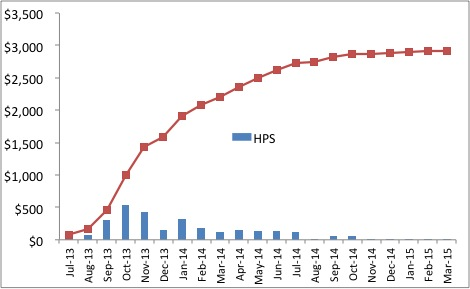
\includegraphics[width=0.9\textwidth]{cost_schedule/spending} 
\caption{Spending profile (costs after overheads and contingency).}
\label{fig:spending_profile}
\end{figure}

\subsection{Schedule}
Our goal is to be ready to install the HPS at JLab by September 2014, and to proceed with commissioning on beam early in FY2015. Data taking 
would begin in Spring 2015 and last until Summer. Meeting this schedule has required keep-alive funding at SLAC for the period April-September, 2013, 
to begin critical long leadtime engineering and prototyping, and it will need  approval and funding from DOE by the beginning of FY2014. Schedules 
for each of the major subsystems of the experiment are given in Figures \ref{fig:schedulea}, \ref{fig:scheduleb} and \ref{fig:schedulec}, and summarized here. The total construction schedule extends over 16 months, 
assuming the funding becomes available in October 2014. The schedule contingency is about 20\%.
 
The conceptual design of the beamline will be done during calendar 2013. Formal beamline engineering will start when funding is secured. A Beamline Engineering 
Design Review will be held in December 2013 to validate the concept before committing funds to construction. 
Final Engineering and Construction will start in Spring 2014 and will be completed well before the installation time in October 2014, providing substantial float. 

Using keep-alive funds, the Test Run SVT was shipped back to SLAC in early February 2013 for continued commissioning of the SVT DAQ, reworking the 
modules for the first three layers of the HPS, and commissioning the motion control systems. The engineering design and prototyping of the Layers 1-2-3 and 
Layers 4-5-6 has already begun using keep alive funding. An Engineering Design Review of the SVT will be held late in fiscal 2013, before major construction
begins. 

Engineering for the new SVT DAQ has also begun. An Engineering Review will precede major construction.  Integrating the SVT DAQ with the SVT and commissioning the
entire system will occur in Spring 2014. The SVT will be ready for shipping in June 2014, and be ready for installation at JLab by mid-August 2014.  Installing 
the SVT in the analyzing magnet vacuum chamber on beamline will likely occur in September, depending on the schedule at JLab.  The SVT schedule has 1 month of 
float between the shipping and the test at JLab, which provides additional contingency for the construction work at SLAC.

The Ecal work will start when funding is received early in FY2014 and will run through June 2014. The scheduled work is relatively minor, so the ECAL will 
easily be ready for installation by August 2014. In the event supplemental funding is received from France or Italy, the construction work will be more ambitious, 
with the possible addition of new APDs and/or new preamplifiers. However, experienced teams at INFN Genova and Orsay already have familiarity with the proposed
improvements, and can straightforwardly manage the construction in time for the installation at JLab.

The schedule includes a series of milestones to track the progress of each subsystem, given in Table \ref{tb:milestones}. These milestones will help HPS management monitor the readiness of each 
sub-detector or system after initial assembly and testing at the respective assembly sites, and the readiness for installation at JLab.  
Also, ad-hoc Engineering Design Reviews, summarized in Table \ref{tb:reviews}, will be conducted by the Project Manager for each subsystem before major costs are incurred.

%New Milestones table goes here
%planned reviews table goes next 
 
\begin{table}[htdp]
\caption{Project Milestones.}
\begin{center}
\begin{tabular}{|c|c|c|}
\hline
WBS & Milestones & Date\\
\hline\hline

1.1	&Beamline	&1-Mar-13\\
\hline
1.1.13	&Beamline Installed	&1-Mar-13\\
\hline
1.2	&SVT	&11-Mar-13\\
\hline
1.2.3	&Layer 1-3 Ready	&17-Feb-14\\
\hline
1.2.5	&Layer 4-6 Ready	&18-Apr-14\\
\hline
1.2.14	&SVT tested and ready for shipment	&9-Jun-14\\
\hline
1.2.16	&SVT Ready For Installation	&15-Aug-14\\
\hline
1.3	&SVT DAQ	&1-Mar-13\\
\hline
1.3.12	&FE Board Tested w/ hybrid	&5-Aug-13\\
\hline
1.3.15	&Flange DAQ Tested	&10-Jan-14\\
\hline
1.3.14	&DAQ Full system Test	&2-Jun-14\\
\hline
1.3.4.9	&Single Hybrid qualification	&20-Jan-14\\
\hline
1.3.13	&Flex Cable w/ hybrid \& FE board	&10-Jan-14\\
\hline
1.4	&ECAL	&2-Sep-13\\
\hline
1.4.8	&ECAL Ready for the installation	&1-Aug-14\\
\hline
1.7	&Installation \& Commissioning	&4-Aug-14\\
\hline
1.7.5	&HPS ready for the beam	&1-Sep-14\\
\hline
\hline
\end{tabular}
\end{center}
\label{tb:milestones}
\end{table}%

\begin{table}[htdp]
\caption{Planned Review.}
\begin{center}
\begin{tabular}{|c|l|c|}
\hline
WBS&Engineering Reviews& Data\\
\hline
\hline
1.1.2 &	Beamline  Review&	20-Dec-14\\
\hline
1.2.2	&SVT Design Review	&20-Aug-13\\
\hline
1.1.11&	Installation Review	&18-Aug-14\\
\hline
\hline
\end{tabular}
\end{center}
\label{tb:reviews}
\end{table}%

\begin{figure}[H]
\centering
%\vspace*{-5mm}
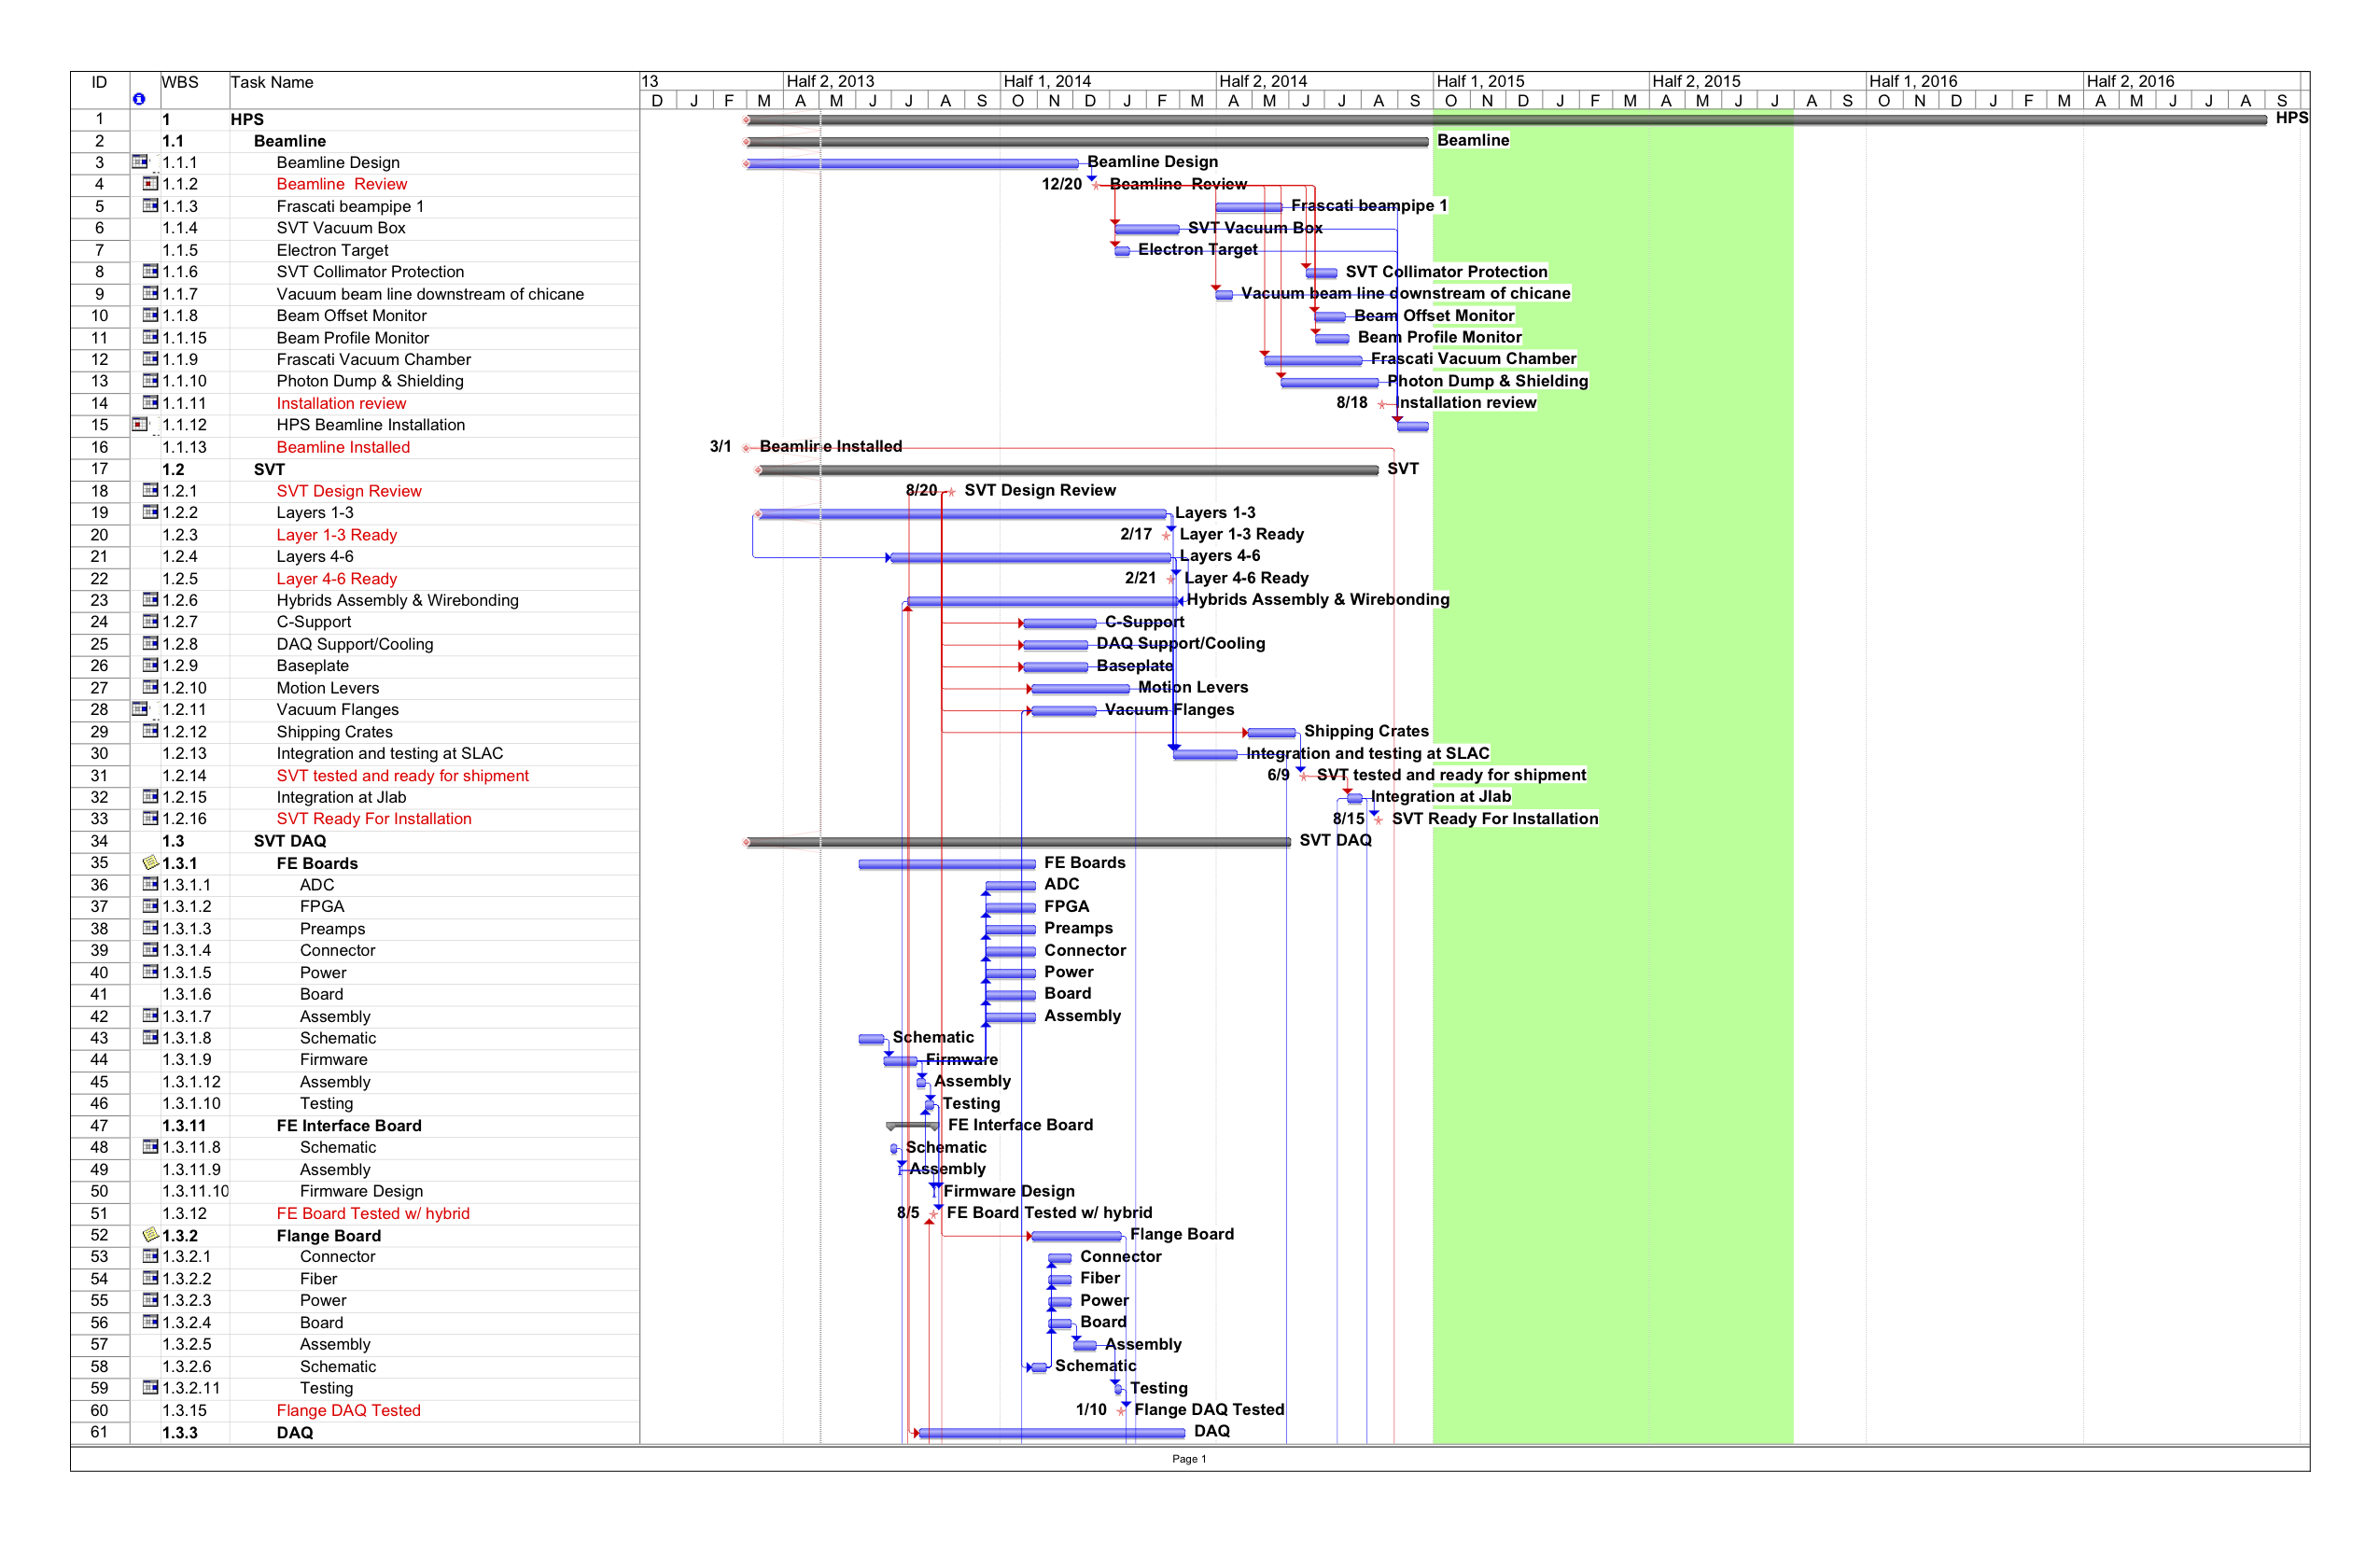
\includegraphics[angle=90,width=0.75\textwidth]{cost_schedule/ScheduleHPSV470-1.jpg} 
\caption{HPS schedule.}
\label{fig:schedulea}
\end{figure}

\begin{figure}[H]
\centering
%\vspace*{-5mm}
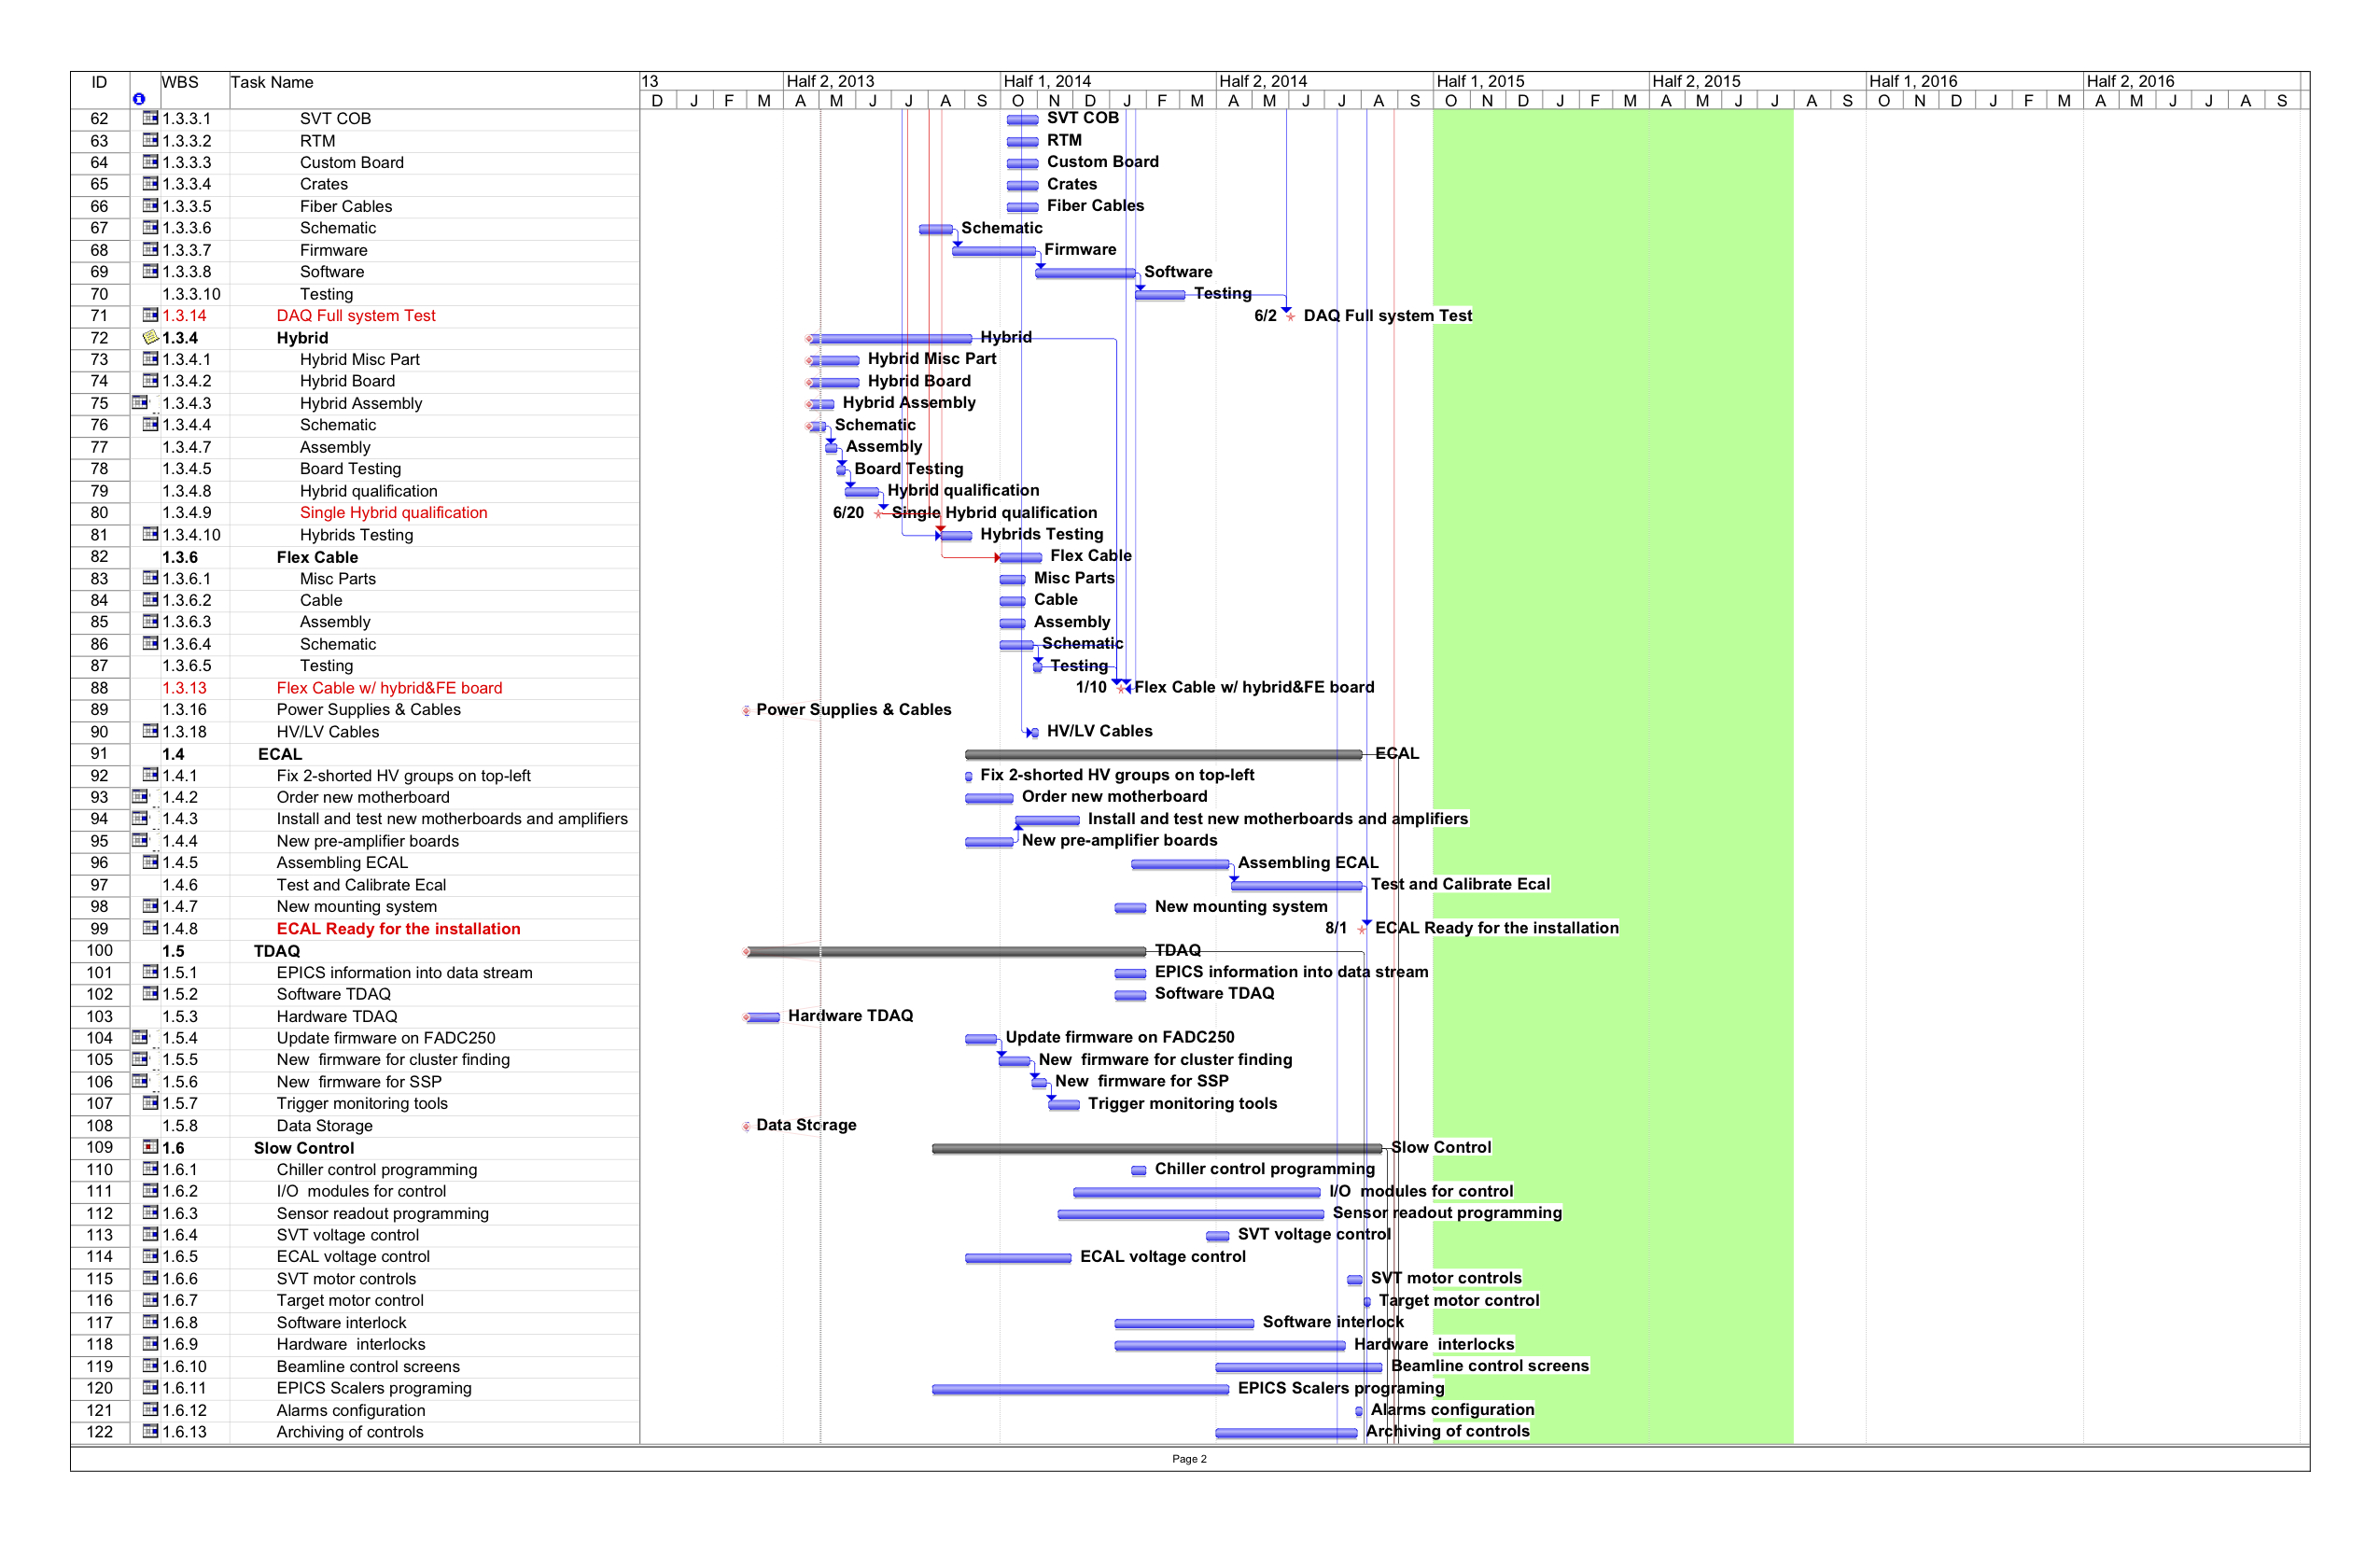
\includegraphics[angle=90,width=0.85\textwidth]{cost_schedule/ScheduleHPSV470-2.jpg} 
\caption{HPS schedule.}
\label{fig:scheduleb}
\end{figure}

\begin{figure}[H]
\centering
%\vspace*{-5mm}
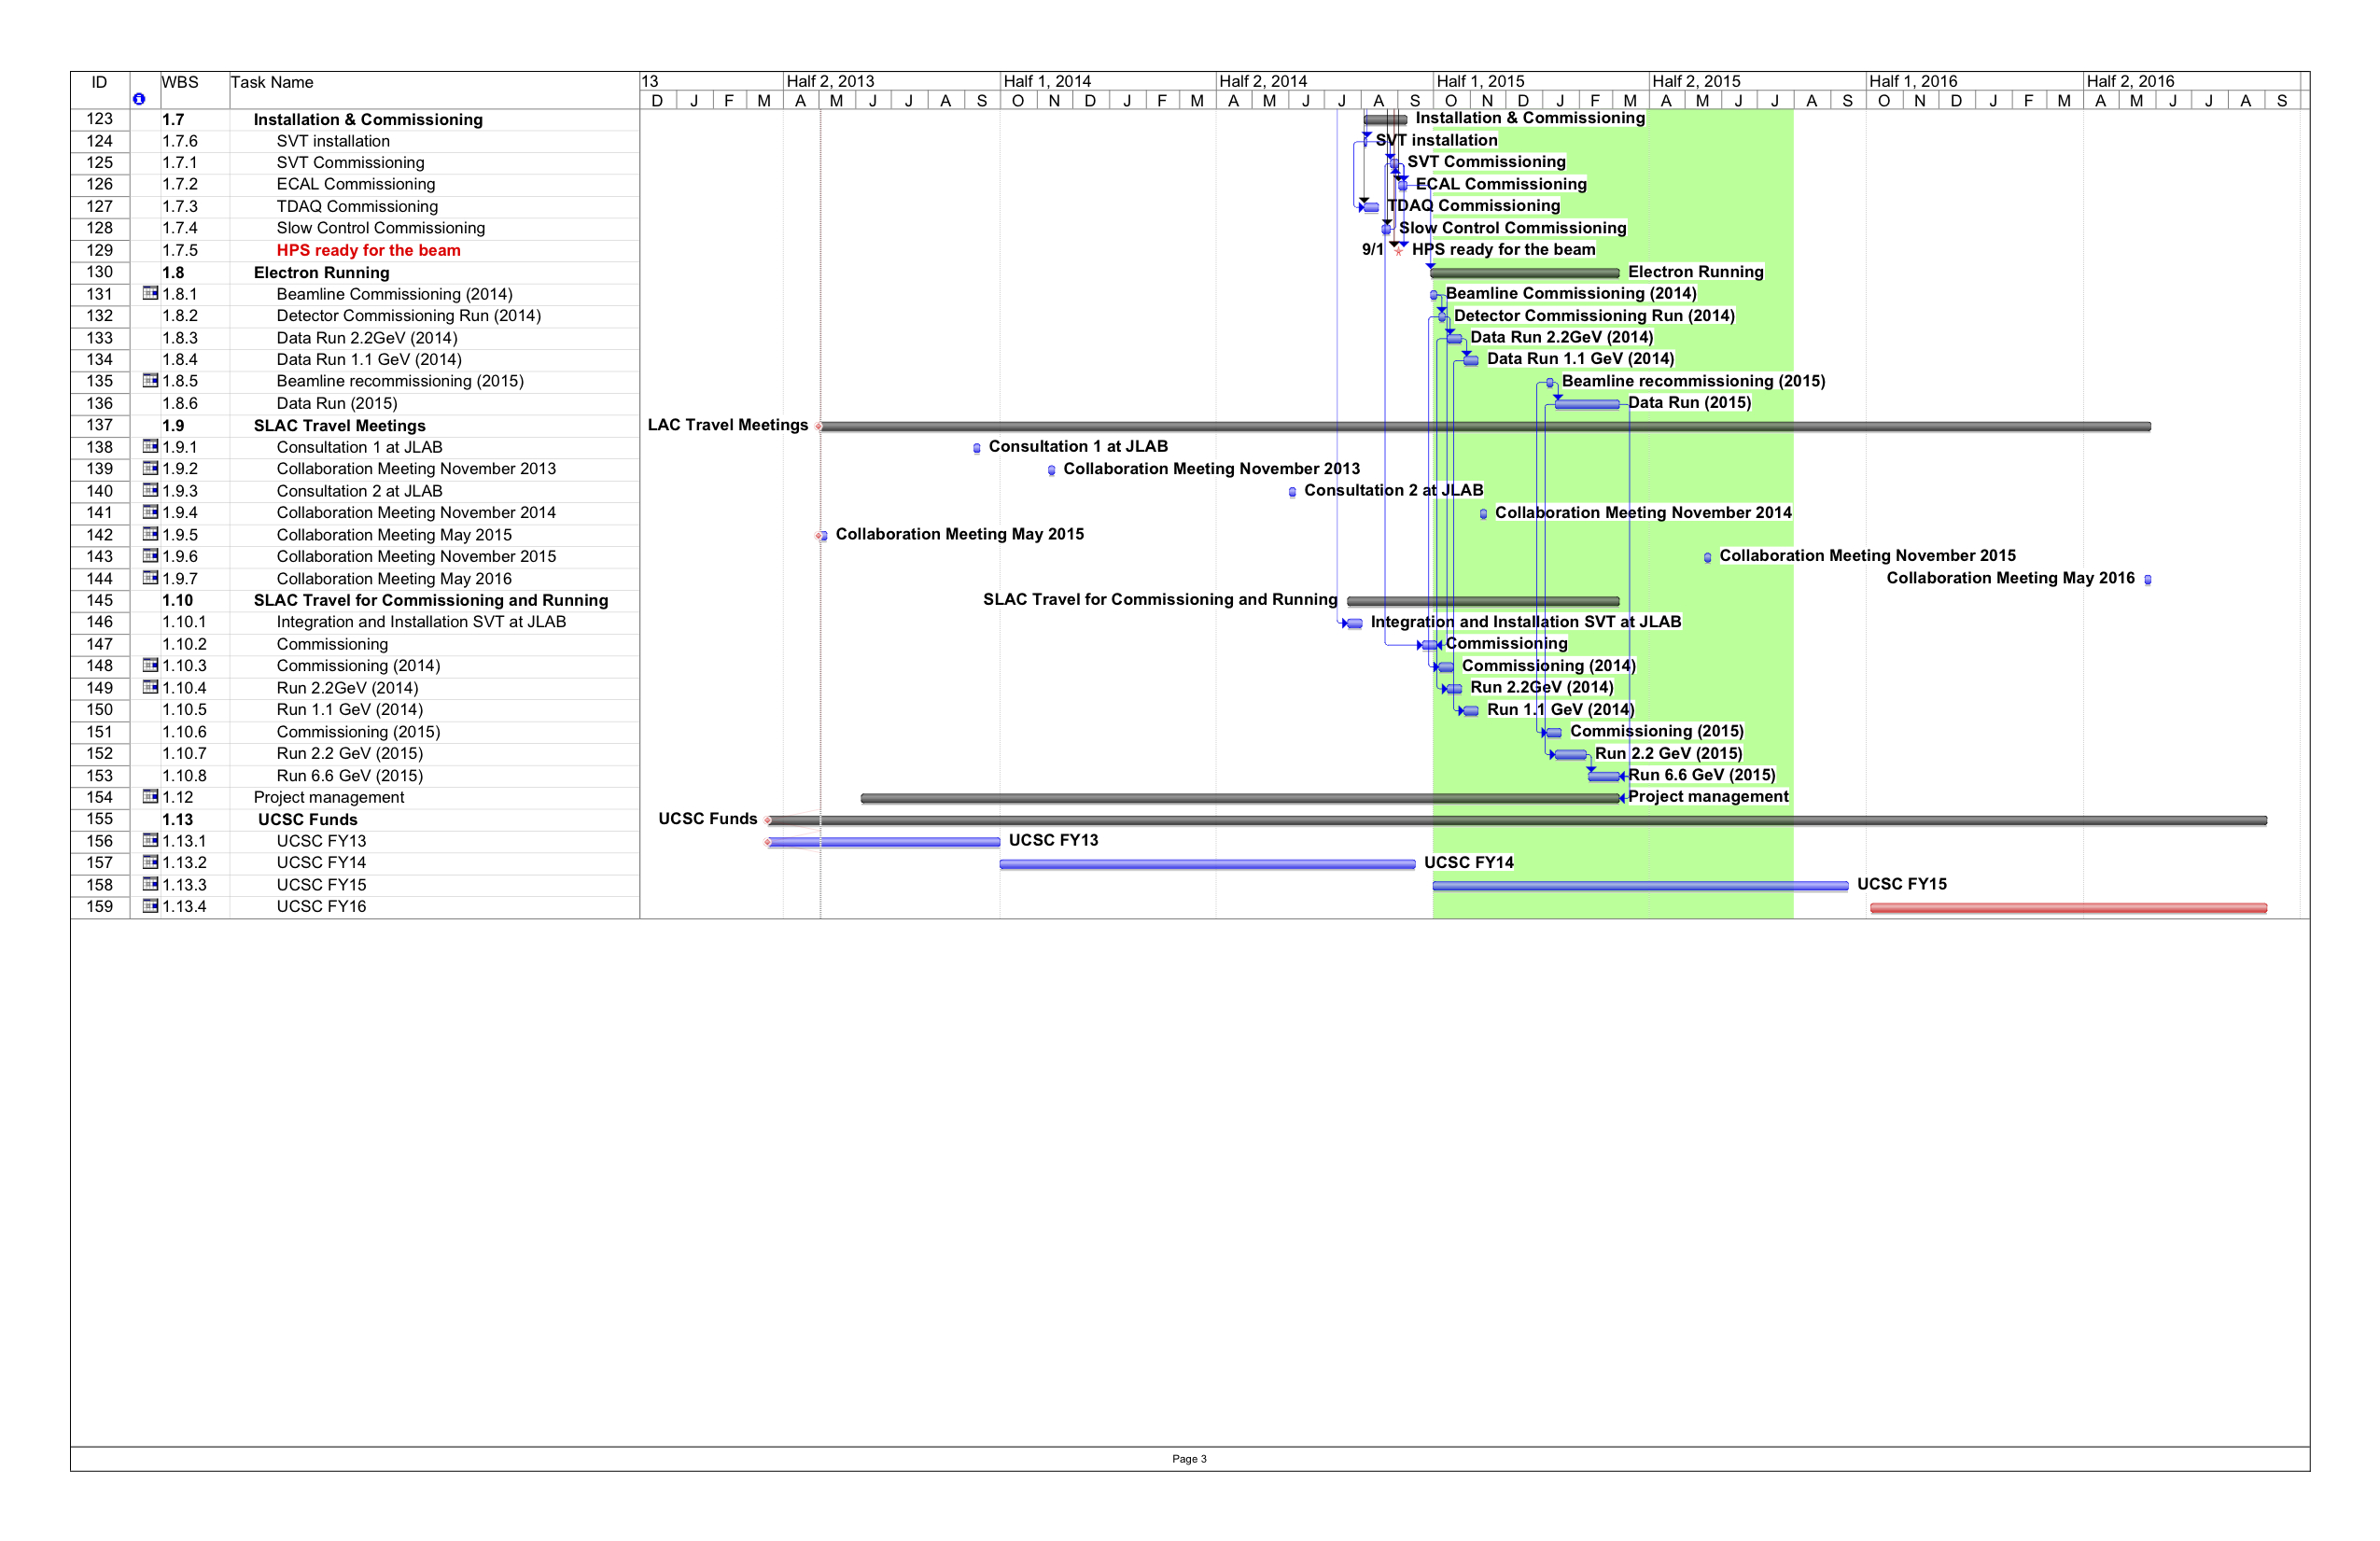
\includegraphics[angle=90,width=0.85\textwidth]{cost_schedule/ScheduleHPSV470-3.jpg} 
\caption{HPS schedule.}
\label{fig:schedulec}
\end{figure}

\subsection{Manpower}

The manpower needed to design, fabricate, assemble, test, install, and commission the HPS is captured in the WBS tables. 
The HPS Collaboration successfully mounted the HPS Test Run experiment on a very aggressive schedule, and has the personnel needed to realize full HPS.

Beamline conceptual design will be done at JLab by Arne Freyberger, F-X Girod and Stepan Stepanyan and at SLAC by Ken Moffeit. 
Mechanical design will be done at JLab.
Engineering at SLAC will be done by Marco Oriunno, Clive Field, and Takashi Maruyama. Fabrication will be done in the 
JLab shops, and installation by the crews at JLab. 

The Tracker/Vertexer is being designed and engineered by Marco Oriunno, Matt Swift, Tim Nelson, and Per Hansson, with additional help 
from Vitaliy Fadeyev, Alex Grillo, and Bill Cooper, all well-experienced with silicon detector systems. Others at SLAC and UCSC will 
help with assembly and testing, including Matt Graham, Takashi Maruyama, John Jaros, and 
graduate students Sho Uemura and Omar Moreno. Matt McCulloch will serve as the technician at SLAC.

The SVT DAQ is being done by Haller's group at SLAC, including Gunther Haller, Ryan 
Herbst, Ben Reese, and Tung Phan, coordinated by physicist Per Hansson. SVT Physicists Alex Grillo, Vitaliy Fadeyev, and Tim Nelson will collaborate closely. 
Graduate students Omar Moreno and Sho Uemura will work with Per Hansson and Ryan Herbst to debug, test, and certify the SVT DAQ electronics.

The Ecal work is being coordinated by the Orsay Group, especially Philippe Rosier, Emmanuel Rindel, Emmanuel Rauly, Raphael Dupre, and Michel Guidal, 
with participation by the JLab group, especially Stepan Stepanyan, and F.-X. Girod.  Others at JLab and in the collaboration will help in 
assembly and test of the ECal, especially the group from INFN Genova (Italy).

The Ecal Trigger/DAQ work is done in Sergey Boyarinov's group, which supports Hall B activities at JLab, and with Chris Cuevas's group, which has designed the FADC250.
R. Dupre and  V. Kubarovsky will collaborate with this group in assembling and testing the electronics, programming the trigger, and integrating it with 
the Ecal hardware. Sho Uemura will test the trigger in simulation, and help develop diagnostics to ensure proper operations.

Slow control programming is being done by Nerses Gevorgyan (Yerevan) and Hovanes Egiyan (JLab).

The HPS collaboration is about 60 strong, so has adequate manpower for overall installation, commissioning, and data taking. Simulation work is supported by Maurik Holtrop, 
Matt Graham, Maurizio Ungaro, Takashi Maruyama, and students Sho Uemura and Omar Moreno. Norman Graf and Jeremy McCormick at SLAC support the lcsim 
simulation/reconstruction framework that is used for HPS simulation and analysis . Data management and storage and computing infrastructure will be overseen by 
Sergey Boyarinov, Maurik Holtrop, Homer Neal, all very experienced professionals, and graduate student Sho Uemura. Analysis and simulation studies have been 
initiated by Maurik Holtrop, Sarah Philips, Joey Reichert, Yuri Gershtein, Matt Graham, Per Hansson, Sho Uemura, Takashi Maruyama, and Omar Moreno. 
Students are actively being engaged.

The total technical labor needed for HPS, divided by category for each of SLAC and JLab, over the next three years, is given in Table \ref{tb:engin}.

\begin{table}[htdp]
\caption{Total Labor (FTE).}
\begin{center}
\parbox{.45\linewidth}{
\begin{tabular}{c||cccc}
\multicolumn{5}{c}{SLAC}\\
 FTE	&FY13	&FY14	&FY15&	FY16\\
 \hline\hline
ME	&0.19	&0.64&	0.14&	0.02\\
MD&	0.09	&0.30&	0.00&	0.00\\
MT&	0.08	&0.49&	0.00	&0.00\\
EE &	0.58	&0.76&	0.05	&0.02\\
ET&	0.01	&0.04&	0.00	&0.00\\
\end{tabular}
%\end{center}
}
\parbox{.45\linewidth}{
%\begin{center}
\begin{tabular}{c||cccc}
\multicolumn{4}{c}{JLab}\\
 FTE	&FY13	&FY14	&	FY15&FY16\\
 \hline\hline
ME	&0.00	&0.03&	0&0 \\
MD&	0.05	&0.06&	0 &0\\
MT&	0.00	&0.14& 0&0\\
EE &	0.12	&1.19&0&0\\
ET&	0.02	&0.07&0&0\\
\end{tabular}
}
\end{center}
\label{tb:engin}
\end{table}%

\subsection{Project Management}

The HPS Collaboration formally came into existence in October, 2011 with the acceptance of Collaboration Bylaws and an initial list of members.
Figure \ref{fig:org_chart} shows the HPS Organization Chart. The HPS Collaboration is managed by its three spokespersons, Maurik Holtrop, John Jaros, and 
Stepan Stepanyan in consultation with the HPS Executive Committee, 
which consists of the spokespeople along with Takashi Maruyama, Matt Graham, Tim Nelson, and F-X Girod. John Jaros serves as Chair of the Executive Committee. 
Ten working groups, shown in Table \ref{tb:groups}, have been created and Chairs and Deputies appointed with responsibilities 
to oversee design, schedule, and budget of each sub-system. 

The overall HPS Project Manager is Marco Oriunno. The Project Management team, Oriunno, Stepanyan, and Jaros,
in consultation with the Executive Committee, has the responsibility to redirect funding as needed to deal with budget and scheduling exigencies.

%add a new figure showing the org chart
\begin{figure*}[ht]
\centering
%\vspace*{-5mm}
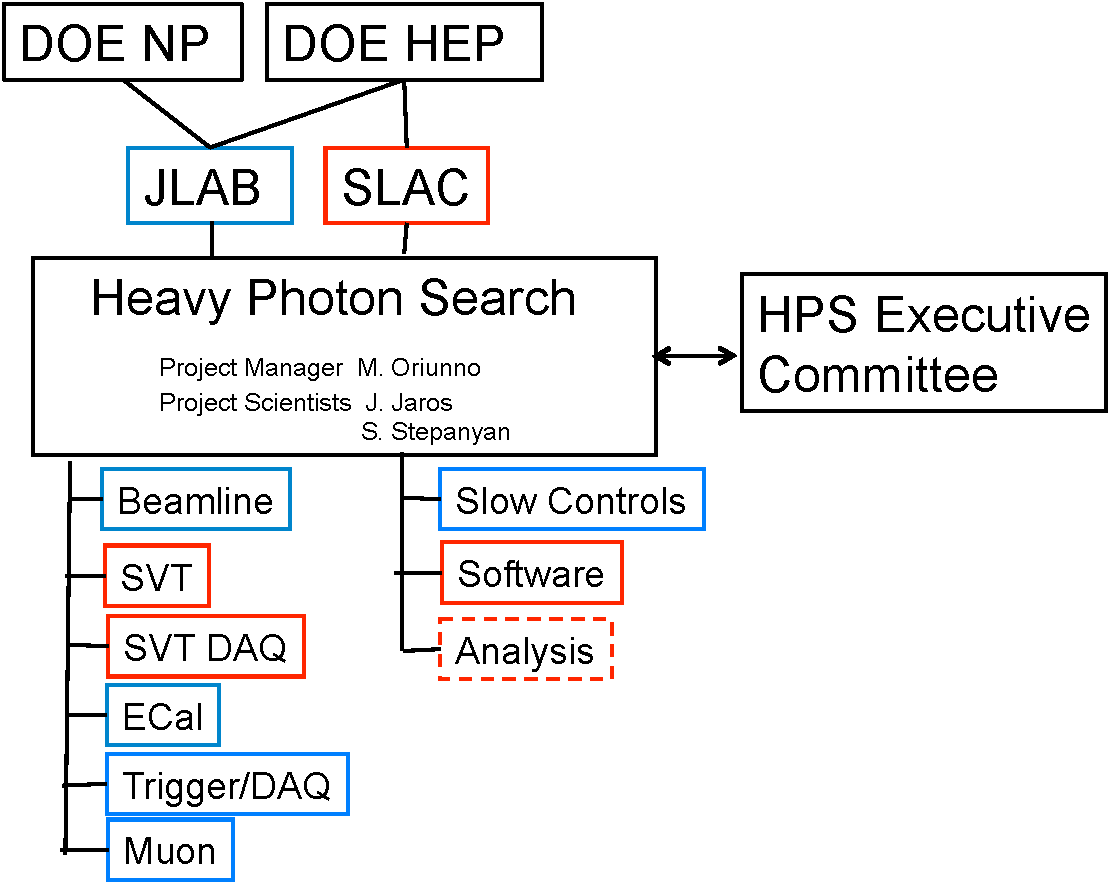
\includegraphics[width=0.9\textwidth]{cost_schedule/org_chart} 
\caption{HPS Organization Chart.}
\label{fig:org_chart}
\end{figure*}

%add Table XXII showing the working groups.

\begin{table}[htdp]
\caption{Working groups.}
\begin{center}
\begin{tabular}{|c|c|c|}
\hline
HPS working Groups	& Chair (Deputy)\\
\hline\hline
Beamline	&K. Moffeit (FX Girod)\\
\hline
SVT	&T. Nelson (V. Fedayev)\\
\hline
ECAL	& R. Dupre (S. Stepanyan)\\
\hline
DAQ	 & S. Boiarinov (P. Hansson)\\
\hline
Trigger &	V. Kubarovsky (T. Maruyama)\\
\hline
Slow Control	& H. Egiyan (N. Gevorgyan)\\
\hline
Muon &	K. Griffioen (Y. Gershtein)\\
\hline
Software	& M. Holtrop (S. Uemura, O. Moreno)\\
\hline
Analysis &	M. Graham (S. Philips)\\
\hline
Project Management &	M. Oriunno (S. Stepanyan, J. Jaros)\\
\hline
\end{tabular}
\end{center}
\label{tb:groups}
\end{table}%

